\section{Work and Kinetic Energy\footnote{1990-93 Dept. of Physics and Astronomy, Dickinson College. Supported by FIPSE
(U.S. Dept. of Ed.) and NSF. Portions of this material have been modified locally
and may not have been classroom tested at Dickinson College.}}

Name \rule{2.0in}{0.1pt}\hfill{}Section \rule{1.0in}{0.1pt}\hfill{}Date \rule{1.0in}{0.1pt}

\textbf{Objectives }

\begin{itemize}
\item To extend the intuitive notion of work as physical effort to a formal mathematical
definition of work as a function of force and distance. 
\item To discover Hooke's law. 
\item To understand the concept of kinetic energy and its relationship to work as
embodied in the work-energy theorem.
\end{itemize}

\textbf{Apparatus }

\begin{center}
\begin{tabular}{lll}
spring scale            & variety of masses & support rod to hand spring\\
wooden block with hook  & large spring      & 2-meter stick \\
\end{tabular}
\end{center}

\textbf{The Concept of Physical Work }

Suppose you are president of the Richmond Load 'n' Go Co. A local college has
three jobs available and will allow you to choose which one you want before
offering the other two jobs to rival companies. All three jobs pay the same
amount of money. Which one would you choose for your crew? 
\textbf{NOTE:} The quantities in this figure are given in British units, 
where ``pounds'' = $mg$, not just $m$, i.e. the $g$ is already included.

\vspace{0.3cm}
{\par\centering 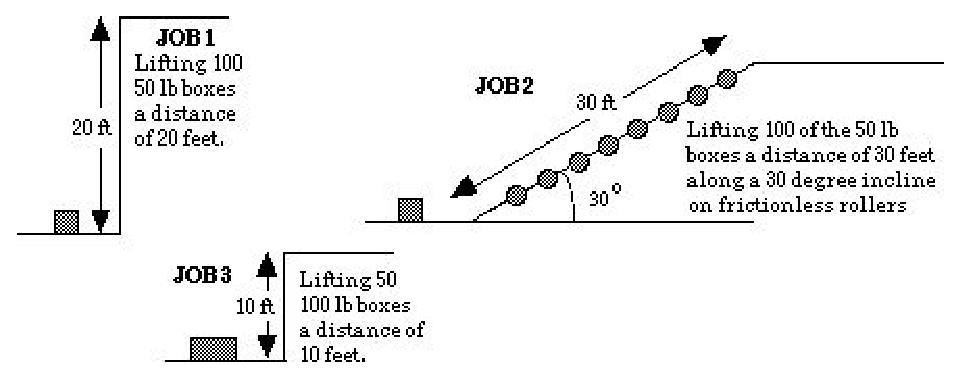
\includegraphics{workAndKE/work_power_fig1.eps} \par}
\vspace{0.3cm}

\textbf{Activity  \stepcounter{activity}\arabic{activity}: Choosing Your Job }

Examine the descriptions of the jobs shown in figure above. Which one would
you be most likely to choose? Least likely to choose? Explain the reasons for
your answer.
\vspace{30mm}

You obviously want to do the least amount of work for the most money. Before
you reconsider your answers later in this unit, you should do a series of activities
to get a better feel for what physicists mean by work and how the president
of Load 'n' Go can make top dollar.

\vspace{0.3cm}
{\par\centering 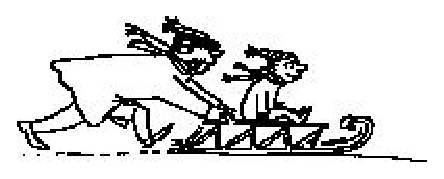
\includegraphics{workAndKE/work_power_fig2.eps} \par}
\vspace{0.3cm}

In everyday language we refer to doing work whenever we expend effort. In order
to get an intuitive feel for how we might define work mathematically, you should
experiment with moving your textbook back and forth along a table top and a
rougher surface such as a carpeted floor.

\textbf{Activity  \stepcounter{activity}\arabic{activity}: This is Work!} 

(a) Pick a distance of a meter or so. Sense how much effort it takes to push
a heavy book that distance. How much more effort does it take to push it twice
as far? 
\vspace{20mm}

(b) Pile another similar book on top of the original one and sense how much
effort it takes to push the two books through the distance you picked. Comment
below.
\vspace{20mm}

(c) If the ``effort'' it takes to move an object is associated
with physical work, guess an equation that can be used to define work mathematically
when the force on an object and its displacement (i.e., the distance it moves)
lie along the same line.
\vspace{20mm}

In physics, work is not simply effort. In fact, the physicist's definition of
work is precise and mathematical. In order to have a full understanding of how
work is defined in physics, we need to consider its definition in a very simple
situation and then enrich it later to include more realistic situations.

\textbf{A Simple Definition of Physical Work:} If an object that is moving in
a straight line experiences a constant force in the direction of its motion
during the time it is undergoing a displacement, the work done by the external
force, \( F_{ext} \), is defined as the product of the force and the displacement of the object, 
\[
W=F_{ext}\Delta x\]


where $W$ represents the work done by the external force, \( F_{ext} \) is the
magnitude of the force, and \( \Delta  x\) is the displacement of the object.
%WHY THE HECK DO WE SAY THIS:
%{\bf I WANT TO DROP THIS SENTENCE:} Work done by a force is always positive!

What if the force of interest and the displacement are in opposite directions? For instance, what about the work done by the force of sliding friction,
\( F_{f} \), when a block slides on a rough surface? The work done by the friction force is
\[
W_{f}=-F_{f}\Delta x\]
%YUCK:
%{\bf AND THIS ONE:} Work done against a force is always negative!

\newpage

\textbf{Activity  \stepcounter{activity}\arabic{activity}: Applying the Physics Definition of Work} 

(a) Does effort necessarily result in physical work? Suppose two guys are in
an evenly matched tug of war. They are obviously expending effort to pull on the
rope, but according to the definition of physical work, are they doing any physical
work? Explain.

\vspace{0.3cm}
{\par\centering 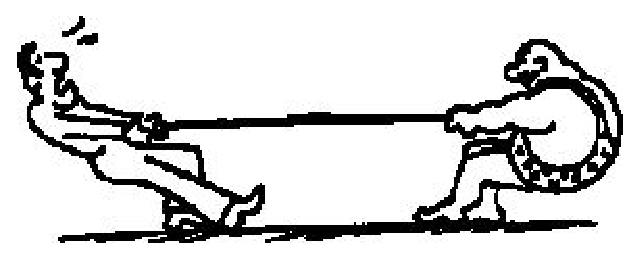
\includegraphics{workAndKE/work_power_fig3.eps} \par}
\vspace{0.3cm}

(b) A wooden block with a mass of 0.30 kg is pushed along a sheet of ice that
has no friction with a constant external force of 10 N which acts in a horizontal
direction. After it moves a distance of 0.40 m how much work has been done on
the block by the external force?
\vspace{20mm}

(c) The same wooden block with a mass of 0.30 kg is pushed along a table with
a constant external force of 10 N which acts in a horizontal direction. It moves
a distance of 0.40 m. However, there is a friction force opposing its motion with magnitude 
$|{\bf F}_{friction}| = \mu N$ where $N$ is the normal force exerted on the block by by the table.
Here $N$ is perpendicular to the surface of the table and equal to the weight of the block (since the table
is holding up the block).
The coefficient of sliding friction $\mu$ is an experimental factor that relates $N$ to the friction force.
Here \( \mu _{k} \), is 0.20. 

\vspace{0.3cm}
{\par\centering 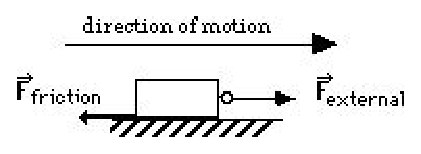
\includegraphics{workAndKE/work_power_fig4.eps} \par}
\vspace{0.3cm}

\begin{enumerate}
\item According to the definition of work done by a force, what is the work associated with the external force? 
Is the work positive or negative? Show your calculation.\vspace{20mm}

\item According to our discussion above of the work done by a friction force, 
what is the work associated with the friction force? 
Is the work positive or negative? Show your calculation.\vspace{20mm}

\end{enumerate}

\newpage

(d) Suppose you lift a 0.3 kg object through a distance of 1.0 m at a constant velocity.

\vspace{0.3cm}
{\par\centering 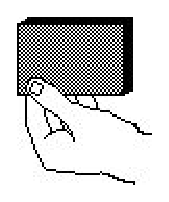
\includegraphics{workAndKE/work_power_fig5.eps} \par}
\vspace{0.3cm}

\begin{enumerate}
\item What is the work associated with the force that the earth exerts on the object? Is the work positive or negative? Show your calculation.
\vspace{20mm}

\item What is the work associated with the external force you apply to the object? Is the work positive or negative? Show your calculation.
\vspace{20mm}

\end{enumerate}
\textbf{Pulling at an Angle What Happens When the Force and the Displacement
Are Not Along the Same Line? }

Let's be more quantitative about measuring force and distance and calculating
the work. How should work be calculated when the external force and the displacement
of an object are not in the same direction?

\vspace{0.3cm}
{\par\centering 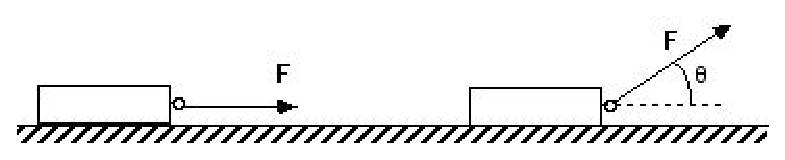
\includegraphics{workAndKE/work_power_fig6.eps} \par}
\vspace{0.3cm}

To investigate this, you will use a spring scale to measure the force necessary
to slide a block along the table at a constant speed. Before you make your simple 
force measurements, you should put some weights on your block so that it slides 
along a smooth surface at a constant velocity even when it is being pulled with 
a force that is 30 or 60 degrees from the horizontal.

\textbf{Activity  \stepcounter{activity}\arabic{activity}: Calculating Work} 

(a) Hold a spring scale horizontal to the table and use it to pull the block
a distance of 0.5 meters along the horizontal surface in such a way that the
block moves at a constant speed. Record the force in newtons and the distance
in meters in the space below and calculate the work done on the block in joules.
(Note that there is a special unit for work, the joule, or J for short. 
One joule is equal to one newton times one meter, i.e., J = N\,m.)
\vspace{20mm}

\newpage

(b) Repeat the measurement, only this time pull on the block at a 30\( ^{\circ } \) 
angle with respect to the horizontal. 
Pull the block at about the same speed. Is the force needed larger or smaller than you measured in part (a)?
\vspace{20mm}

(c) Repeat the measurement once more, this time pulling the block at a 60\( ^{\circ } \) 
angle with respect to the horizontal.  
Pull the block at about the same speed as before.
\vspace{20mm}

(d) Assuming that the actual physical work done in part (b) is the same as the
physical work done in part (a) above, how could you enhance the mathematical
definition of work so that the forces measured in part (b) could be used to
calculate work? In other words, use your data to postulate a mathematical equation
that relates the physical work, $W$, to the magnitude of the applied force, $F$,
the magnitude of the displacement, \( \Delta  s\), and the angle, \( \theta  \),
between $F$ and \( \Delta  s\). Explain your reasoning. Hint: sin 30\( ^{\circ } \)
= 0.500, sin 60\( ^{\circ } \) = 0.866, cos 30\( ^{\circ } \) = 0.866, cos 60\( ^{\circ } \)
= 0.500.
\vspace{20mm}

\textbf{Work as a Dot Product }

Review the definition of dot (or scalar) product as a special product of two
vectors in your textbook, and convince yourself that the dot product can be
used to define physical work in general cases when the force is constant but
not necessarily in the direction of the displacement resulting from it. 
\[W={\bf F}\cdot {\bf \Delta s}\]


\textbf{Activity  \stepcounter{activity}\arabic{activity}: How Much Work Goes with Each Job? }

(a) Re-examine the descriptions of the jobs shown in the figure on the first
page of this experiment. What is the minimum physical work done in job 1? Note that the
 data are given in British units, so the work will be expressed in foot pounds (ft lbs), 
not newton meters. 
Remember, the ``pounds'' are $mg$, so you don't need to multiply by $g$.
\vspace{12mm}

(b) What is the minimum physical work done in job 2?
\vspace{12mm}

(c) What is the minimum physical work is done in job 3?
\vspace{12mm}

(d) Was your original intuition about which job to take correct? Which job should
Richmond Load 'n' Go try to land?
\vspace{12mm}

%----------------------------------------------------------------------------------------

\newpage

\textbf{The Force Exerted on a Mass by an Extended Spring} 

So far we have pushed and pulled on an object with a constant force and calculated
the work needed to displace that object. In most real situations the force on
an object can change as it moves. 

What happens to the average force needed to stretch a spring from 0 to 1 cm
compared to the average force needed to extend the same spring from 10 to 11
cm? How does the applied force on a spring affect the amount by which it stretches,
i.e., its displacement?

\textbf{Activity  \stepcounter{activity}\arabic{activity}: Are Spring Forces Constant?} 

Hang the spring from a support rod with the large diameter coils in the downward
position. Extend the spring from 0 to 1 cm. Feel the force needed to extend
the spring. Extend the spring from 10 to 11 cm. Feel the force needed to extend
the spring again. How do the two forces compare? Are they the same? 
\vspace{10mm}

\textbf{The Force and Work Needed to Stretch a Spring} 

Now we would like to be able to quantify the force and work needed to extend
a spring as a function of its displacement from an equilibrium position (i.e.,
when it is ``unstretched'').

\textbf{Activity  \stepcounter{activity}\arabic{activity}: Force vs. Displacement for a Spring }\actlabel{hooke}

(a) The table below shows the results of a series of measurements of the distance $s$ from the floor to
the position of a mass $m$ hung from a spring like the one you have.
Calculate and record the external force, \( F_{ext} \), 
and the stretch of the spring, \(x\) (\(= s_{0} - s\)), for each mass.
The last four columns will not be filled in until you get to Activities \ref{forceDistance} and \ref{work}.

\begin{center}
\begin{tabular}{|c|c|c|c|c|c|c|c|c|} \hline
$m$ (kg) & $s$ (m) & $ F_{ext} $ (N)  & $x$ (m) & $\Delta x$ (m) & $\langle x\rangle$ (m) & $\langle F_{ext}\rangle $ (N) & $\Delta W$ (J) & $ W_{total}$ (J) \\ \hline
0.0      &  1.508  &                 &         &                &                        &                               &                &                  \\ \hline
0.1      &  1.390  &                 &         &                &                        &                               &                &                  \\ \hline
0.2      &  1.220  &                 &         &                &                        &                               &                &                  \\ \hline
0.3      &  1.153  &                 &         &                &                        &                               &                &                  \\ \hline
0.4      &  1.032  &                 &         &                &                        &                               &                &                  \\ \hline
0.5      &  0.911  &                 &         &                &                        &                               &                &                  \\ \hline
0.6      &  0.789  &                 &         &                &                        &                               &                &                  \\ \hline
0.7      &  0.669  &                 &         &                &                        &                               &                &                  \\ \hline
0.8      &  0.547  &                 &         &                &                        &                               &                &                  \\ \hline
0.8      &  0.420  &                 &         &                &                        &                               &                &                  \\ \hline
1.0      &  0.301  &                 &         &                &                        &                               &                &                  \\ \hline
\end{tabular}
\end{center}

(b) Using \textit{Excel}, create a graph of \( F_{ext} \) (vertical axis) vs. $x$. 
Is the graph linear?
If the force, \( F_{ext} \), increases with the displacement in a proportional
way, fit the data to find the slope of the line. Insert a copy of the graph
into your notebook. Use the symbol $k$ to represent the slope of the line. What
is the value of $k$? What are its units? Note: 
$k$ is known as the spring constant.
\vspace{10mm}

(c) Write the equation describing the relationship between the external force,
\( F_{ext} \), and the total displacement, 
$x$, of the spring from its equilibrium
using the symbols \( F_{ext} \), $k$, and $x$.
\vspace{10mm}

Note: Any restoring force on an object which is proportional to its displacement
is known as a Hooke's Law Force. There was an erratic, contentious genius named
Robert Hooke who was born in 1635. He played with springs and argued with Newton.

\newpage

\textbf{Calculating Work when the Force is not Constant }

We would like to expand the definition of work so it can be used to calculate
the work associated with stretching a spring and the work associated with other
forces that are not constant. A helpful approach is to plot the average force
needed to move an object for each successive displacement \( \Delta  x\) as
a bar graph like that shown in the figure below. The figure shows a graph representing
the average applied force causing each unit of displacement of an object. This
graph represents force that is not constant but not the force vs. displacement
of a typical spring.

Note: The bar graph below is intended to illustrate mathematical concepts. Any
similarity between the values of the forces in the bar graph and any real set
of forces is purely coincidental. In general, the force causing work to be done
on an object is not constant.

\vspace{0.3cm}
%{\par\centering \includegraphics{work_kinetic_fig1.eps} \par}
{\par\centering 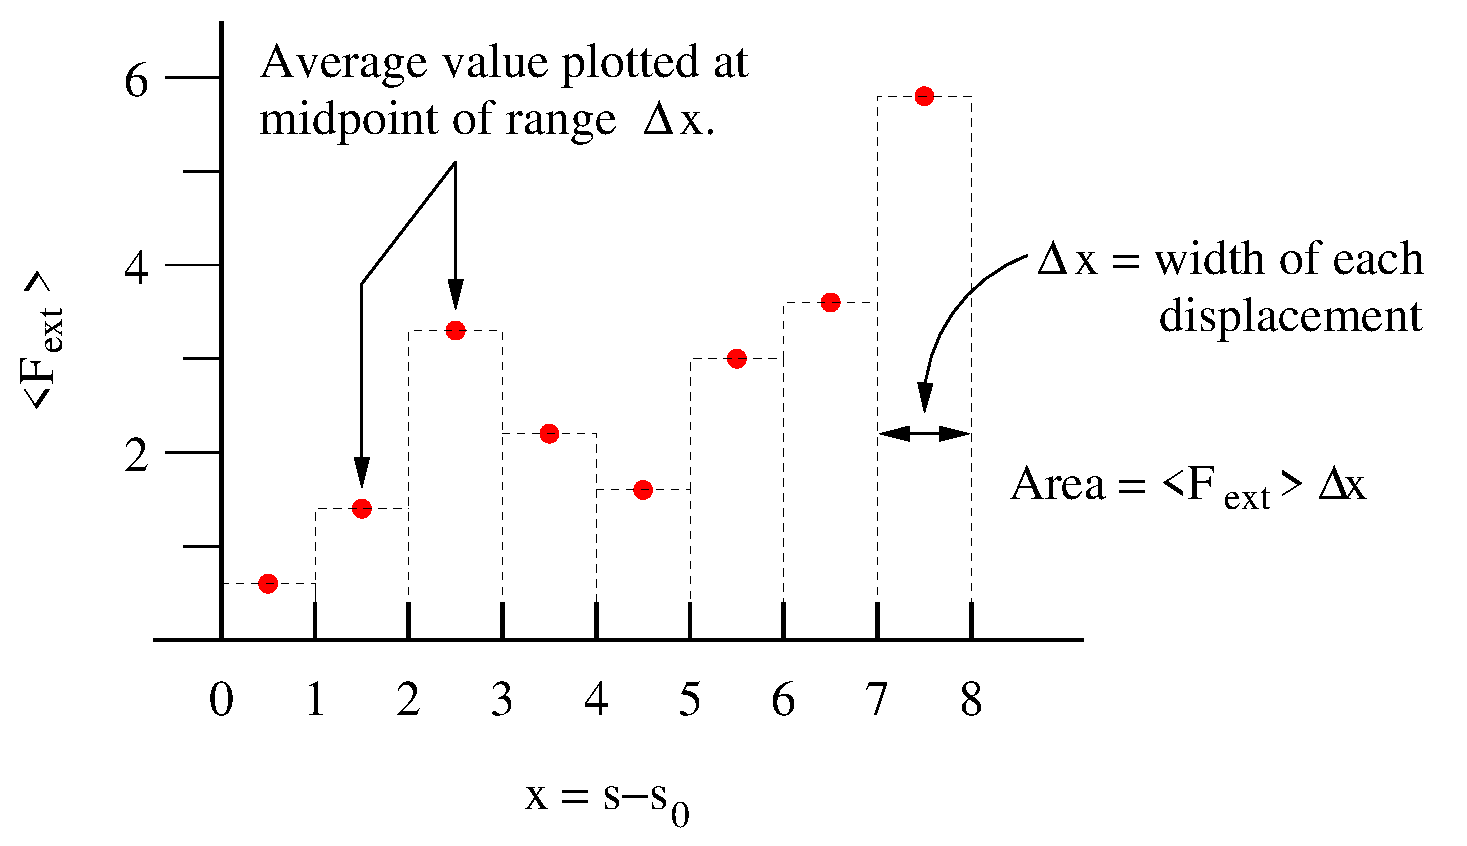
\includegraphics[width=6.0in]{workAndKE/workAndKEF1.eps} \par}
\vspace{0.3cm}

\textbf{Activity  \stepcounter{activity}\arabic{activity}: Force vs. Distance in a Bar Graph }\actlabel{forceDistance}

(a) Using your data from Activity \ref{hooke}, calculate the width of each displacement \( \Delta x \),
the average position for each displacement $\langle x \rangle$, 
and the average external force \(\langle F_{ext} \rangle\) for each displacement, 
and record the values in the table above. Plot \( \langle F_{ext} \rangle\) vs. $x$ 
as a bar graph on the grid below.  
(Choose appropriate scales for the axes before making the graph.)

\vspace{0.3cm}
%{\par\centering \includegraphics{work_kinetic_fig2.eps} \par}
{\par\centering 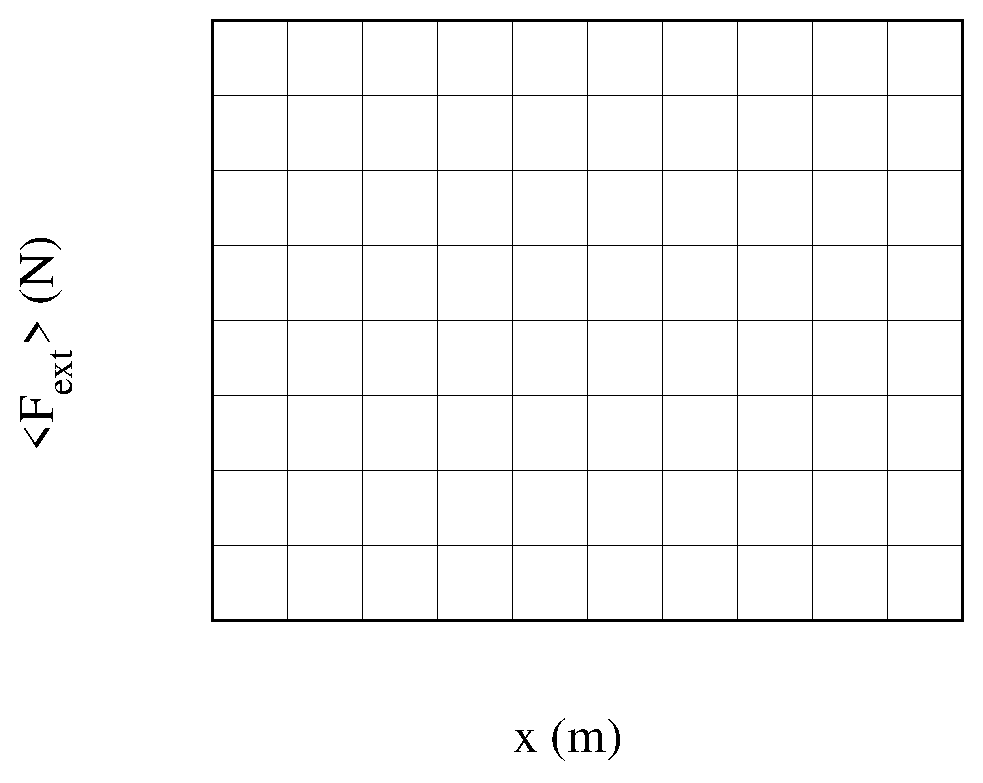
\includegraphics[width=6.0in]{workAndKE/workAndKEF2.eps} \par}
\vspace{0.3cm}

How can we calculate the work done in stretching the spring? We can use several
equivalent techniques: (1) adding up little pieces of \( \langle F_{ext} 
\rangle \Delta x \) from the above bar graph,
(2) finding the area under the ``curve'' you created in Activity \ref{hooke}, or (3)
using mathematical integration.

All three methods should yield about the same result. 
If you have studied integrals in calculus you may want to consult
your instructor or the textbook about how to set up the appropriate definite
integral to calculate the work needed to stretch the spring. 

\textbf{Activity  \stepcounter{activity}\arabic{activity}: Calculation of Work }\actlabel{work}

(a) Calculate the work needed to stretch the spring by adding up small increments of 
\( \langle F_{ext} \rangle \Delta  x\) (this is \( \Delta W\)) in your table. 
Also record the running sum in the table and indicate the final value of \( W_{total} \) below. 
Don't forget to specify units.
\vspace{5mm}

\( W_{total} =\) 
\vspace{5mm}

(b) Calculate the work needed to stretch the spring by computing the area under
the curve in the graph of \( F_{ext} \) vs. $x$ that you created in Activity \ref{hooke}.
\vspace{20mm}

\newpage

(c) How does adding up the little rectangles in part (a) compare to finding
the area under the curve in part (b)? 
\vspace{20mm}

Note that in the limit where the $x$ values are very small the sum of 
\(\langle F_{ext} \rangle
\Delta  x\), known by mathematicians as the Riemann sum, converges to the
mathematical integral and to the area under the curve.

\textbf{Defining Kinetic Energy and Its Relationship to Work} 

What happens when you apply an external force to an object that is free to move
and has no friction forces on it? Obviously it should experience an acceleration
and end up being in a different state of motion. Can we relate the change in
motion of the object to the amount of work that is done on it?

Let's consider a fairly simple situation. Suppose an object is lifted through
a distance $s$ near the surface of the earth and then allowed to fall. During
the time it is falling it will experience a constant force as a result of the
attraction between the object and the earth glibly called the force of gravity.
You can use the theory we have already developed for the gravitational force
to compare the velocity of the object to the work done on it by the gravitational
field as it falls through a distance 
$y$. This should lead naturally to the definition
of a new quantity called kinetic energy, which is a measure of the amount of
``motion'' gained as a result of the work done on the mass. 

\textbf{Activity  \stepcounter{activity}\arabic{activity}: Equations for Falling v vs. y }\actlabel{falling}

(a) An object of mass m is dropped near the surface of the earth. What are the
magnitude and direction of its acceleration $g$?
\vspace{10mm}

(b) If the object has no initial velocity and is allowed to fall for a time
$t$ under the influence of the gravitational force, what kinematic equation describes the relationship between the distance the object falls, $y$, and its time of fall, $t$? Assume \( y_{0}=0 \) and take positive down.
\vspace{10mm}

(c) Do you expect the magnitude of the velocity to increase, decrease or remain
the same as the distance increases? Note: This is an obvious question!!
\vspace{10mm}

(d) Differentiate the equation you wrote down in part (b) to find a relationship
between $v$, the acceleration $g$, and time $t$.
\vspace{20mm}

(e) Eliminate $t$ from the equations you obtained in parts (b) and (d) to get
an expression that describes how the velocity, $v$, 
of the falling object depends
on the distance, $y$, through which it has fallen. 
\vspace{20mm}

You can use the kinematic equations to derive the functional relationship you
hopefully discovered experimentally in the last activity. If we define the kinetic
energy ($K$) of a moving object as the quantity $K = {1\over 2}mv^{2}$, then we
can relate the change in kinetic energy as an object falls to the work done
on it. Note that for an object initially at rest the initial kinetic energy
is \(K _{i}=0\), so the change in kinetic energy is given by the difference
between the initial and final kinetic energies. \( \Delta  K = K _{f}
- K_{i}  = {1\over 2}mv^{2} \).

\textbf{Activity  \stepcounter{activity}\arabic{activity}: Computing Work and Kinetic Energy of a Falling Mass} 

(a) Suppose the mass of your falling object is 0.35 kg. What is the value of
the work done by the gravitational force when the mass is dropped through a
distance of $y = 1.2$ m? 
\vspace{20mm}

(b) Use the kinematic equation you derived in Activity \ref{falling}(e) that relates $v$ and
$y$ to find the velocity of the falling object after it has fallen 1.2 m.
\vspace{20mm}

(c) What is the kinetic energy of the object before it is dropped? After it
has fallen 1.2 m? What is the change in kinetic energy, \( \Delta  K\), as
a result of the fall?
\vspace{20mm}

(d) How does the work done by the gravitational force compare to the kinetic
energy change, \( \Delta  K\), of the object?
\vspace{20mm}

\textbf{Activity  \stepcounter{activity}\arabic{activity}: The Mathematical Relationship between Work and Kinetic Energy Change In a Fall }

(a) Since our simplified case involves a constant acceleration, write down the
equation you derived in Activity \ref{falling}(e) to describe the speed, $v$, of a falling
object as a function of the distance $y$ which it fell.
\vspace{10mm}

(b) Using the definition of work, show that $W = mgy$ when the object is dropped
through a distance $y$.
\vspace{10mm}

(c) By combining the equations in parts (a) and (b) above, show that in theory
the work done on a mass falling under the influence of the gravitational attraction
exerted on it by the earth is given by the equation \(W = \Delta  K\).
\vspace{20mm}

\newpage

(d) You have just proven an example of the work-energy theorem which states that
the change in kinetic energy of an object is equal to the net work done
by all the forces acting on it.
\[
W=\Delta K\qquad \mbox{[Work-Energy Theorem]}\]


Although you have only shown the work-energy theorem for a special case where
no friction is present, it can be applied to any situation in which the net
force can be calculated. For example, the net force on an object might be calculated as a combination of applied, spring, gravitational, and friction forces.

